\section{Block Chipers}
Block cipher are PRPs families that operate one a block of a fixed length. To ensure security against CPA, there are varius mode of operation for block ciphers, like \emph{Electronic Code Block} (ECB), \emph{Cipher Block Chaining} (CBC), and \emph{Counter Mode} (CTR).

\subsection{Electronic Code Book}
Given a plaintext $m = m_1,...,m_l$, the encryption is obtained by encrypting each block separately: $c = \langle F_k(m_1),...,F_k(m_l) \rangle$.
The decryption is carried out by applying to every block $F_k^{-1}$. Due to the fact that the encryption process is deterministic, repeated blocks will be repeated also in the ciphertext. This mean this mode is not CPA-secure neither have indistinguishable encryption in the presence of a eavesdropper.
\begin{figure}[H]
    \centering
    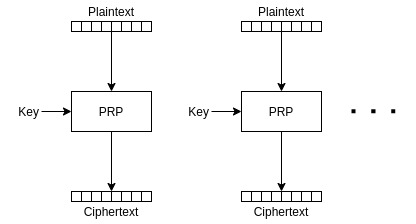
\includegraphics[width=0.6\textwidth]{img/private-key/ecb.jpg}
    \caption{ECB encryption.}
\end{figure}

\subsection{Cipher Block Chaining}
First is an initial vector IV of length n is chosen. So is set $c_0 = IV$ and for every $i > 0$, $c_i := F_k(c_{i-1} \oplus m_i)$. The final ciphertext is $<IV,c_1,...,c_l>$. The IV is not kept secret to allow decription. The encryption of single blocks must be carried out sequentially
\begin{figure}[H]
    \centering
    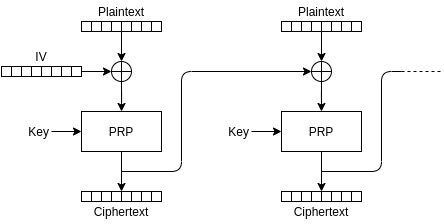
\includegraphics[width=0.6\textwidth]{img/private-key/cbc.jpg}
    \caption{CBC encryption.}
\end{figure}

\subsection{Randomized Counter Mode}
As in CBC, an IV of length n is chosen. Then is computed $r_i := F_k((IV + i)\;\mathsf{mod}\;2^n)$. Then each block of the plaintex is computed as $c_i := r_i \oplus m_i$. Unlike in CBC, with CTR it's possible to encrypt and decrypt in parallel.
\begin{figure}[H]
    \centering
    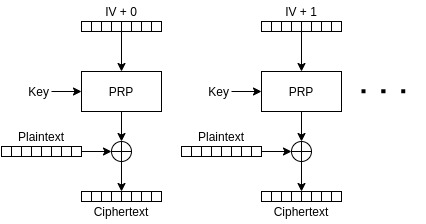
\includegraphics[width=0.6\textwidth]{img/private-key/ctr.jpg}
    \caption{CTR encryption.}
\end{figure}

\begin{figure}[h]
    \centering
    \fbox{
\includegraphics[width=0.2\textwidth]{img/private-key/unimore-original.jpg}}
    \fbox{
\includegraphics[width=0.2\textwidth]{img/private-key/unimore-ecb.jpg}}
    \fbox{
\includegraphics[width=0.2\textwidth]{img/private-key/unimore-ctr.jpg}}
    \fbox{
\includegraphics[width=0.2\textwidth]{img/private-key/unimore-cbc.jpg}}
    \caption{From left to right: original image, image encrypted with ECB, image encrypted with CTR, image encrypted with CBC. It's easy to notice the problem with ECB.}
\end{figure}
